\documentclass{article}
\usepackage[T1]{fontenc}
\usepackage{lmodern}
\usepackage{graphicx}
\usepackage{amsmath,amssymb}
\usepackage[a4paper,margin=2cm]{geometry}
\usepackage[absolute,overlay]{textpos}
\setlength{\TPHorizModule}{1mm}
\setlength{\TPVertModule}{1mm}
\usepackage[indonesian]{babel}
\usepackage{hyperref}
\setlength{\emergencystretch}{2em}
% unit: Halaman 35

\begin{document}

% === Halaman 35 (llm) ===

\vspace{237.60mm}

Demo online: \href{https://www.dcode.fr/columnar-transposition-cipher}{https://www.dcode.fr/columnar-transposition-cipher}

% deskripsi: Screenshot halaman web dCode yang menampilkan alat Decoder dan Encoder untuk Columnar Transposition Cipher, lengkap dengan input teks, kunci permutasi, dan opsi konfigurasi.
% bbox normalisasi: [0.0500, 0.1500, 0.8700, 0.9500]
\begin{textblock*}{172.20mm}(10.50mm,44.55mm)
\noindent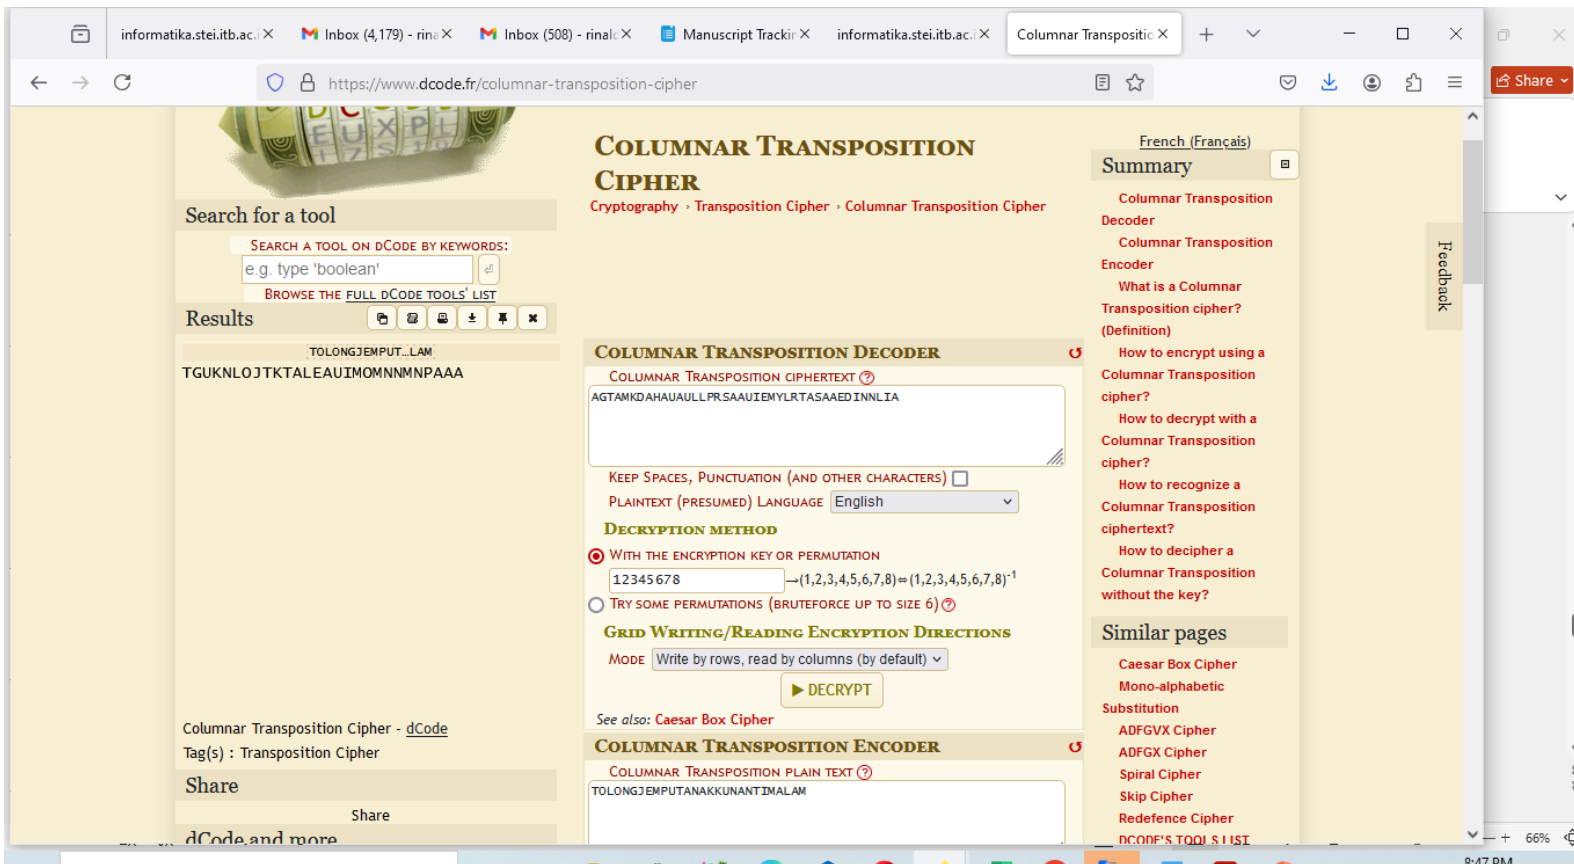
\includegraphics[width=172.20mm,height=237.60mm]{../../images/llm/page_035_img_01.png}%
\end{textblock*}

\end{document}
